\documentclass[border=2pt]{standalone}
\usepackage{tikz}
\usetikzlibrary{arrows.meta,chains,%
                    decorations.pathreplacing}
\usetikzlibrary{matrix,positioning,arrows.meta,arrows}
\usetikzlibrary{calc}

\tikzset{
mymat/.style={
  matrix of nodes,
  nodes in empty cells,
  text height=2.5ex,
  text depth=0.75ex,
  text width=3.25ex,
  align=center,
  column sep=-\pgflinewidth
  },
cartesian/.style={
  align=center, inner sep=1pt, text centered,
  font=\sffamily, circle, black, draw=black, 
  fill=white, text=black, minimum width=0.5em, minimum height=1em
  }
}
\tikzset{
  rows/.style 2 args={
    sub@rows/.style={row ##1 column #2/.style={nodes={rectangle,draw=black}}},
    sub@rows/.list={#1}
  },
  box/.style 2 args={
    sub@box/.style={rows={#1}{##1}},
    sub@box/.list={#2}
  }
}
\begin{document}

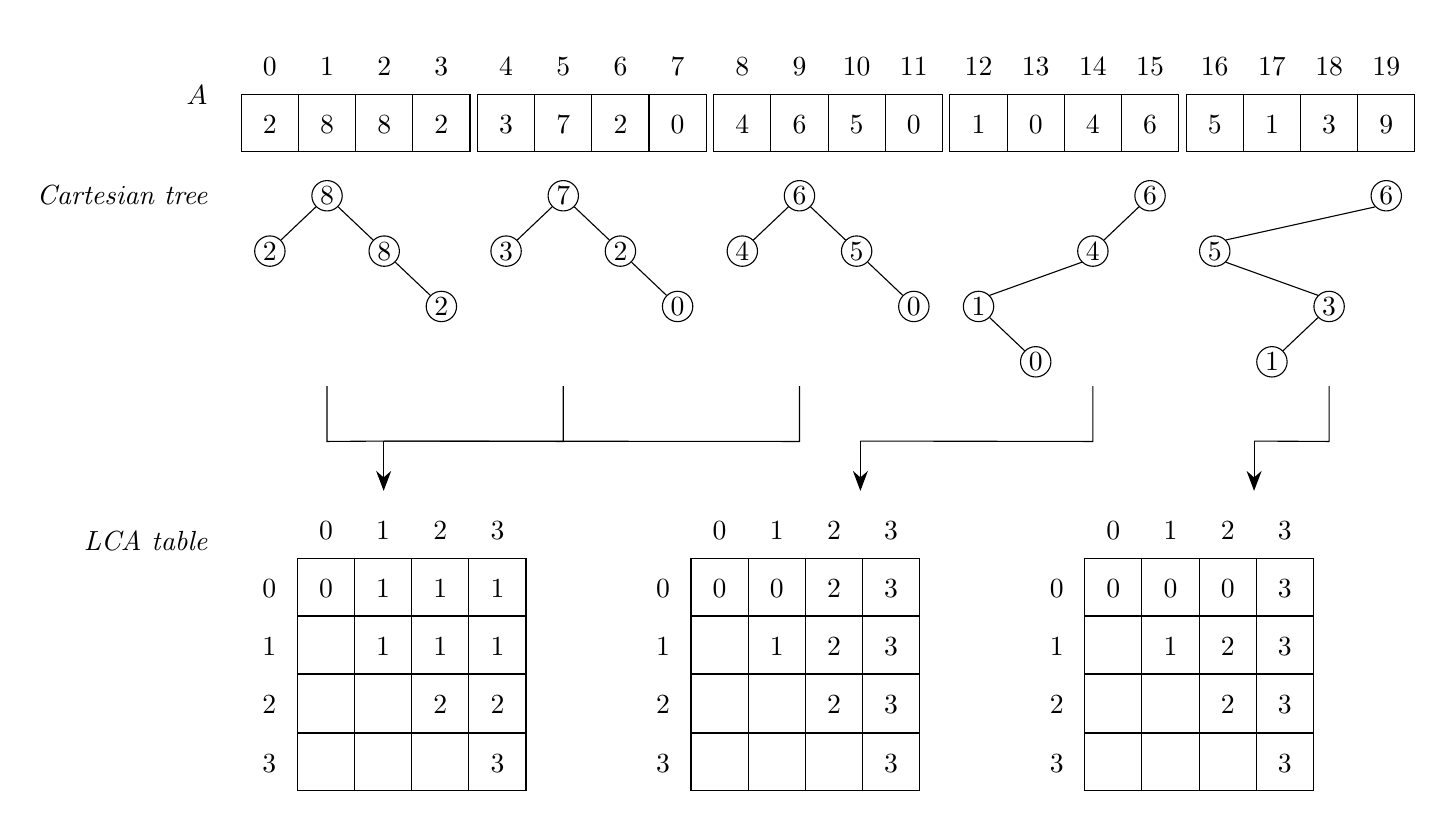
\begin{tikzpicture}[>=latex]
\matrix[mymat,anchor=west,
    box={2}{1, 2, 3, 4}]
at (0,0) 
(mat1)
{ 
  0 & 1 & 2 & 3 \\
  2 & 8 & 8 & 2 \\ };
\matrix[mymat,anchor=west,
    box={2}{1, 2, 3, 4}]
at (3,0) 
(mat2)
{ 4 & 5 & 6 & 7 \\
  3 & 7 & 2 & 0 \\ };
\matrix[mymat,anchor=west,
    box={2}{1, 2, 3, 4}]
at (6,0) 
(mat3)
{ 8 & 9 & 10 & 11 \\
  4 & 6 & 5 & 0 \\ };
\matrix[mymat,anchor=west,
    box={2}{1, 2, 3, 4}]
at (9,0) 
(mat4)
{ 
  12 & 13 & 14 & 15 \\
  1 & 0 & 4 & 6 \\ };
\matrix[mymat,anchor=west,
    box={2}{1, 2, 3, 4}]
at (12,0) 
(mat5)
{ 16 & 17 & 18 & 19 \\
  5 & 1 & 3 & 9 \\ };

\node[left=5pt of mat1]
{
   $A$ \\
};

\node[below left=5pt and 5pt of mat1]
{
   $\textit{Cartesian tree}$ \\
};

\node[below left=130pt and 5pt of mat1]
{
   $\textit{LCA table}$ \\
};


% block 1
\node[cartesian, below=10pt of mat1-2-2.south](B1-1){$8$};
\node[cartesian, below=30pt of mat1-2-3.south](B1-2){$8$};
\node[cartesian, below=30pt of mat1-2-1.south](B1-0){$2$};
\node[cartesian, below=50pt of mat1-2-4.south](B1-3){$2$};

\begin{scope}
\draw[](B1-1.south west) -- (B1-0.north east);
\draw[](B1-1.south east) -- (B1-2.north west);
\draw[](B1-2.south east) -- (B1-3.north west);
\end{scope}

\coordinate(B1tree) at([yshift=-95pt]mat1-2-2);

% block 2
\node[cartesian, below=10pt of mat2-2-2.south](B2-1){$7$};
\node[cartesian, below=30pt of mat2-2-3.south](B2-2){$2$};
\node[cartesian, below=30pt of mat2-2-1.south](B2-0){$3$};
\node[cartesian, below=50pt of mat2-2-4.south](B2-3){$0$};

\begin{scope}
\draw[](B2-1.south west) -- (B2-0.north east);
\draw[](B2-1.south east) -- (B2-2.north west);
\draw[](B2-2.south east) -- (B2-3.north west);
\end{scope}

\coordinate(B2tree) at([yshift=-95pt]mat2-2-2);

% block 3
\node[cartesian, below=10pt of mat3-2-2.south](B3-1){$6$};
\node[cartesian, below=30pt of mat3-2-3.south](B3-2){$5$};
\node[cartesian, below=30pt of mat3-2-1.south](B3-0){$4$};
\node[cartesian, below=50pt of mat3-2-4.south](B3-3){$0$};

\begin{scope}
\draw[](B3-1.south west) -- (B3-0.north east);
\draw[](B3-1.south east) -- (B3-2.north west);
\draw[](B3-2.south east) -- (B3-3.north west);
\end{scope}

\coordinate(B3tree) at([yshift=-95pt]mat3-2-2);

% block 4
\node[cartesian, below=10pt of mat4-2-4.south](B4-3){$6$};
\node[cartesian, below=30pt of mat4-2-3.south](B4-2){$4$};
\node[cartesian, below=50pt of mat4-2-1.south](B4-0){$1$};
\node[cartesian, below=70pt of mat4-2-2.south](B4-1){$0$};

\begin{scope}
\draw[](B4-3.south west) -- (B4-2.north east);
\draw[](B4-2.south west) -- (B4-0.north east);
\draw[](B4-0.south east) -- (B4-1.north west);
\end{scope}

\coordinate(B4tree) at([yshift=-95pt]mat4-2-3);

% block 5
\node[cartesian, below=10pt of mat5-2-4.south](B5-3){$6$};
\node[cartesian, below=30pt of mat5-2-1.south](B5-0){$5$};
\node[cartesian, below=50pt of mat5-2-3.south](B5-2){$3$};
\node[cartesian, below=70pt of mat5-2-2.south](B5-1){$1$};

\begin{scope}
\draw[](B5-3.south west) -- (B5-0.north east);
\draw[](B5-0.south east) -- (B5-2.north west);
\draw[](B5-2.south west) -- (B5-1.north east);
\end{scope}

\coordinate(B5tree) at([yshift=-95pt]mat5-2-3);

% type of a Cartesian tree

\matrix[mymat,anchor=west,
    box={2,3,4, 5}{2, 3, 4, 5}]
at (0,-7) 
(type1)
{ 
    & 0 & 1 & 2 & 3 \\
  0 & 0 & 1 & 1 & 1 \\ 
  1 &   & 1 & 1 & 1 \\ 
  2 &   &   & 2 & 2 \\
  3 &   &   &   & 3 \\};

\matrix[mymat,anchor=west,
    box={2,3,4, 5}{2, 3, 4, 5}]
at (5,-7) 
(type2)
{ 
    & 0 & 1 & 2 & 3 \\
  0 & 0 & 0 & 2 & 3 \\ 
  1 &   & 1 & 2 & 3 \\ 
  2 &   &   & 2 & 3 \\
  3 &   &   &   & 3 \\};

\matrix[mymat,anchor=west,
    box={2,3,4, 5}{2, 3, 4, 5}]
at (10,-7) 
(type3)
{ 
    & 0 & 1 & 2 & 3 \\
  0 & 0 & 0 & 0 & 3 \\ 
  1 &   & 1 & 2 & 3 \\ 
  2 &   &   & 2 & 3 \\
  3 &   &   &   & 3 \\};

% link to table

\coordinate(type1f) at([yshift=18pt]type1.north);

\coordinate(B1treef) at([yshift=-20pt]B1tree.north);
\coordinate(B2treef) at([yshift=-20pt]B2tree.north);
\coordinate(B3treef) at([yshift=-20pt]B3tree.north);
\coordinate(B4treef) at([yshift=-20pt]B4tree.north);
\coordinate(B5treef) at([yshift=-20pt]B5tree.north);

\draw (B1tree) -- (B1treef) -- (type1f);
\draw (B2tree) -- (B2treef) -- (type1f);
\draw (B3tree) -- (B3treef) -- (type1f);
\draw[-{Stealth[scale=1.5]}] (type1f) -- (type1);

\coordinate(type2f) at([yshift=18pt, xshift=30pt]type2.north);
\coordinate(type2b) at([xshift=30pt]type2.north);

\draw (B4tree) -- (B4treef) -- (type2f);
\draw[-{Stealth[scale=1.5]}] (type2f) -- (type2b);

\coordinate(type3f) at([yshift=18pt, xshift=30pt]type3.north);
\coordinate(type3b) at([xshift=30pt]type3.north);

\draw (B5tree) -- (B5treef) -- (type3f);
\draw[-{Stealth[scale=1.5]}] (type3f) -- (type3b);

\end{tikzpicture}

\end{document}